\begin{figure}
  \centering
  \begin{subfigure}[b]{0.5\textwidth}
    \centering
    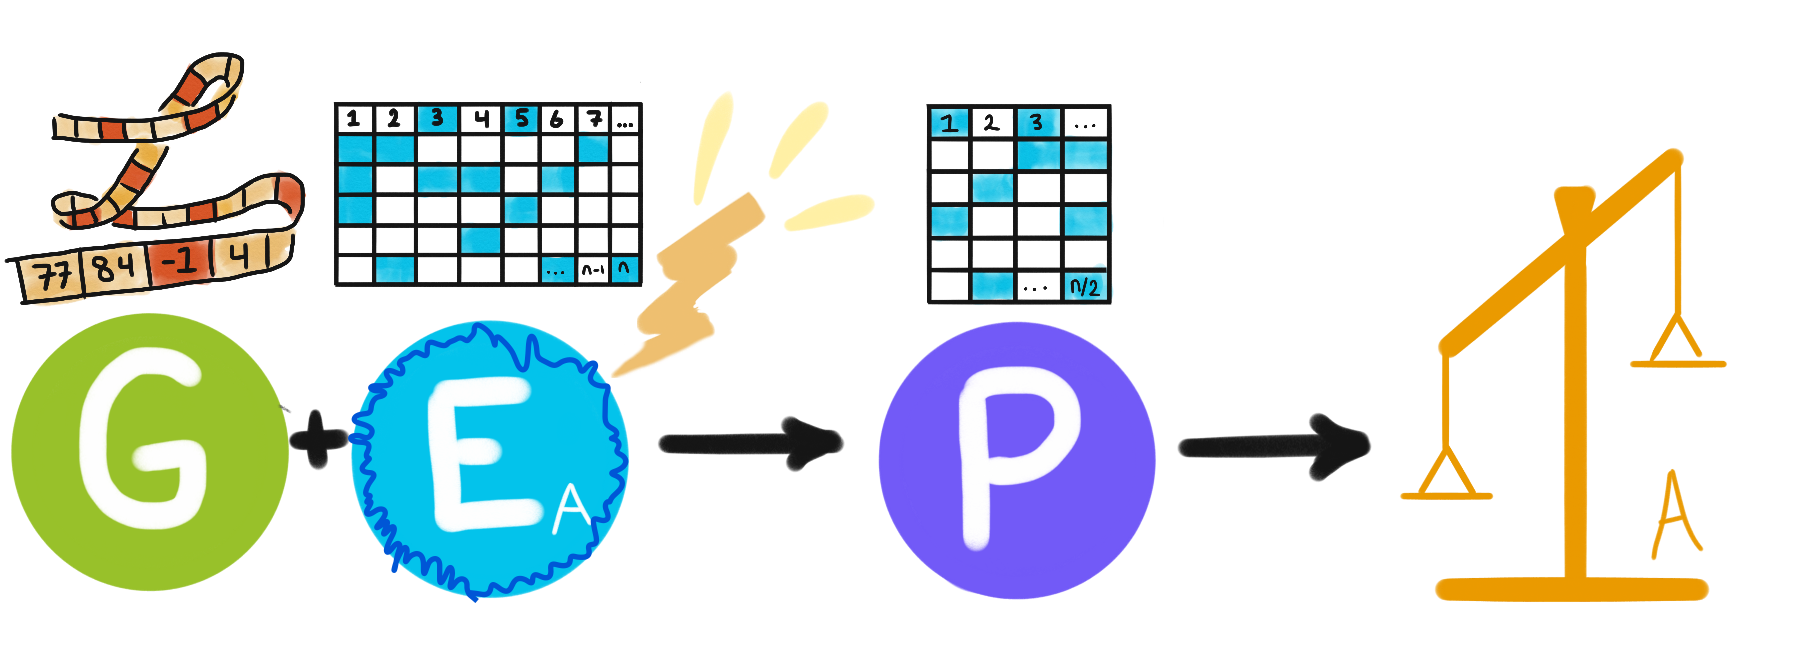
\includegraphics[width=\textwidth]{img/combinedschemeA} \\
    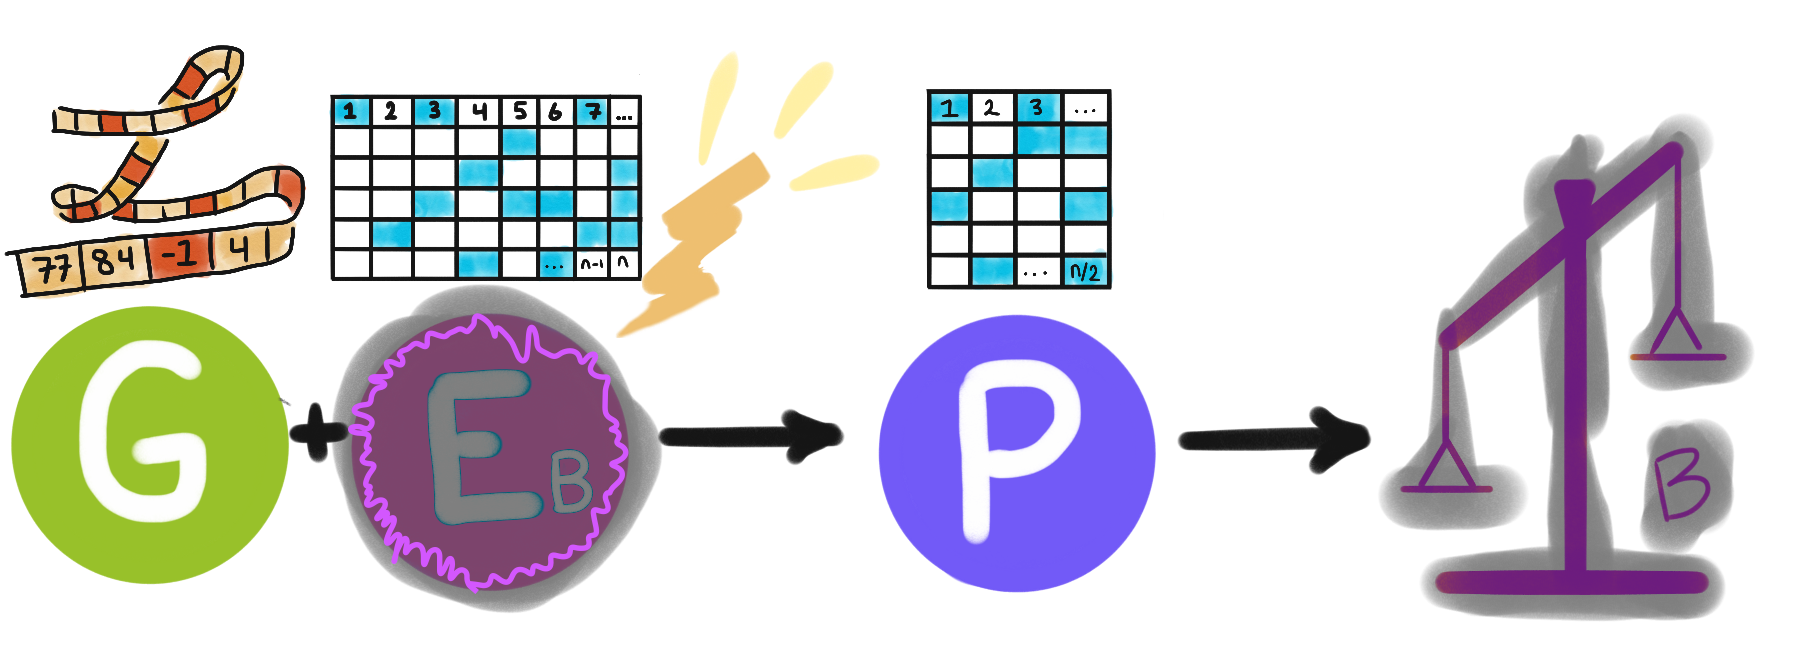
\includegraphics[width=\textwidth]{img/combinedschemeB}
    \caption{experimental scheme}
    \label{subfig:directscheme}
  \end{subfigure}%
  \hfill
  \begin{subfigure}[b]{0.5\textwidth}
    \centering
    
    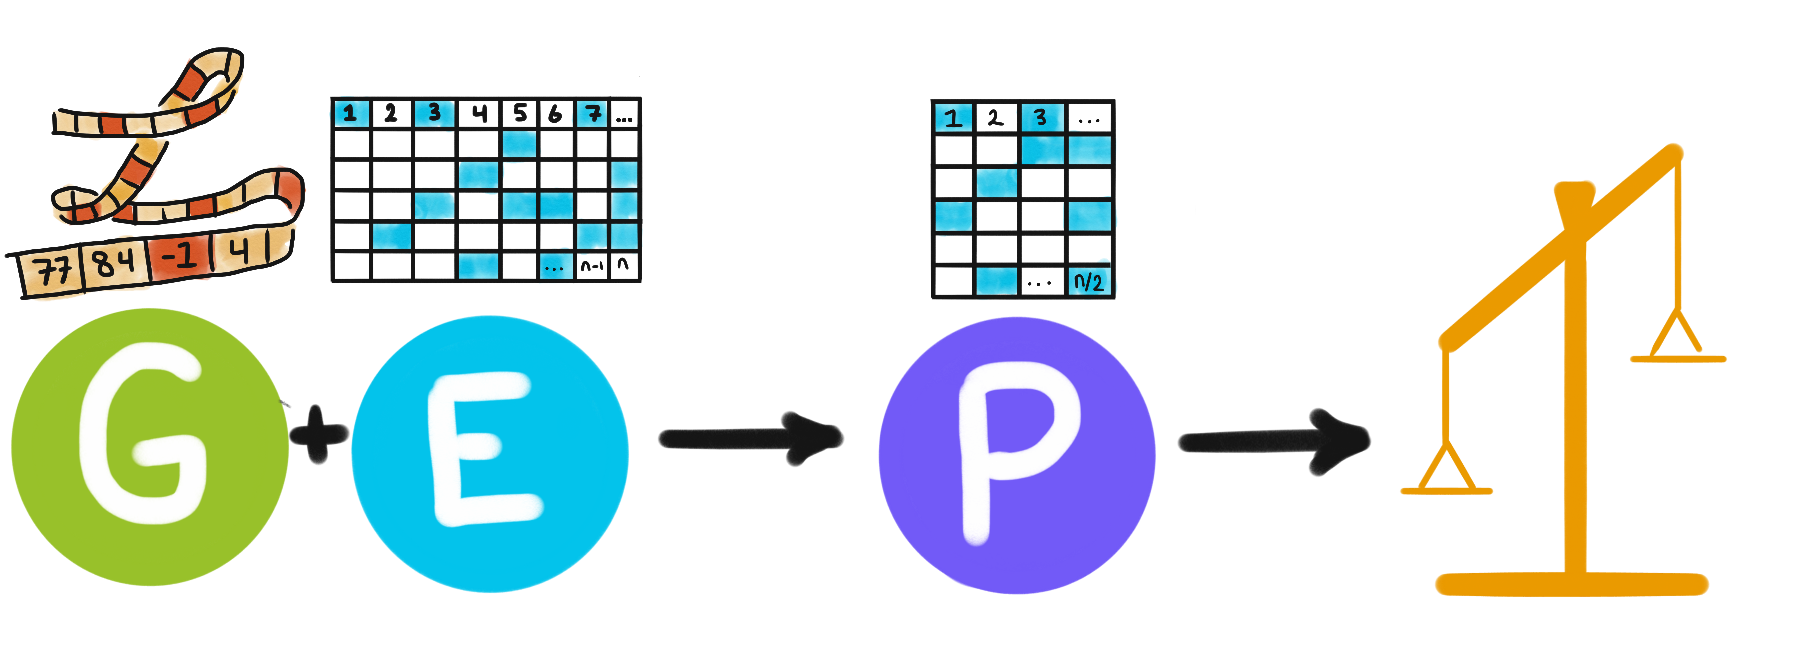
\includegraphics[width=\textwidth]{img/modelscheme} \\
 \vspace{5ex}
    \caption{control scheme}
     \label{subfig:controlscheme}
  \end{subfigure}
  \captionsetup{singlelinecheck=off,justification=raggedright}
  \caption{A comparison of the control and experimental schemes employed to investigate the relationship between combined plasticity and evolvability.}
  \label{fig:combined_plasticity_scheme}
\end{figure}